\documentclass[12pt,a4paper]{beamer}
\usepackage[utf8]{inputenc}
\usepackage[francais]{babel}
\usepackage[T1]{fontenc}
\usepackage{amsmath}
\usepackage{amsfonts}
\usepackage{amssymb}
\usepackage{graphicx}

\begin{document}

%%%%%%%%%%%%%%%%%%%%%%%%%%%%%%%%%%%%%%%%%%%%%%%%%%%%%%%%%%%%%%%%%%%%%%%%%%%%%%%
\begin{frame}
\begin{center}
{\Huge \bf Ecole Polytechnique}\\

\vspace{1cm}

{\LARGE{\bf kNN-CUDA\\ }}
INF560 - Calcul Parallèle et Distribuée

\vspace{1cm}
COELHO LECHNER, Carlos\\
LOBATO GIMENES, Tiago\\
\end{center}

\begin{center}
\textbf{Palaiseau, France \\  Hiver 2014-2015}
\end{center}
\end{frame}

%%%%%%%%%%%%%%%%%%%%%%%%%%%%%%%%%%%%%%%%%%%%%%%%%%%%%%%%%%%%%%%%%%%%%%%%%%%%%%%
\begin{frame}{Vision générale du kNN}
\begin{itemize}
\item \textbf{Définition}: Algorithme qui a comme sortie les k plus proches voisins d'un point requête dans une nuage de points. 
\item \textbf{Utilités}: 
	\begin{itemize}
	\item Apprentissage supervisé
	\item Classification
	\end{itemize}
\end{itemize}
\end{frame}

%%%%%%%%%%%%%%%%%%%%%%%%%%%%%%%%%%%%%%%%%%%%%%%%%%%%%%%%%%%%%%%%%%%%%%%%%%%%%%%
\begin{frame}{Répresentation du kNN}
\begin{figure}
\centering
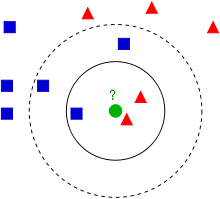
\includegraphics[width=0.3\textwidth]{../figures/KNN.png}
\caption{\label{fig:3KNN} Représentation du 3-KNN.}
\end{figure}
\end{frame}

%%%%%%%%%%%%%%%%%%%%%%%%%%%%%%%%%%%%%%%%%%%%%%%%%%%%%%%%%%%%%%%%%%%%%%%%%%%%%%%
\begin{frame}{L'algorithme}
\begin{itemize}
\item Algorithme en deux étapes:
\begin{itemize}
\item Calcul des distances
\item Triage des distances
\end{itemize}
\end{itemize}
\end{frame}

%%%%%%%%%%%%%%%%%%%%%%%%%%%%%%%%%%%%%%%%%%%%%%%%%%%%%%%%%%%%%%%%%%%%%%%%%%%%%%%
\begin{frame}{Distances}
\begin{figure}
\centering
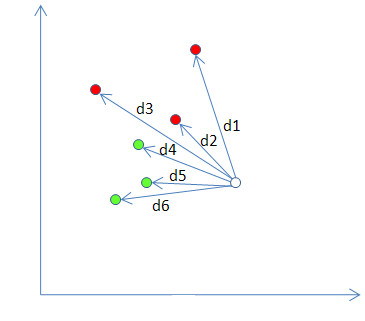
\includegraphics[scale=0.6]{../figures/knn_distances.jpg}
\end{figure}
\end{frame}

%%%%%%%%%%%%%%%%%%%%%%%%%%%%%%%%%%%%%%%%%%%%%%%%%%%%%%%%%%%%%%%%%%%%%%%%%%%%%%%
\begin{frame}{Triage - Bitonic sort} 
\begin{figure}[h]
\centering
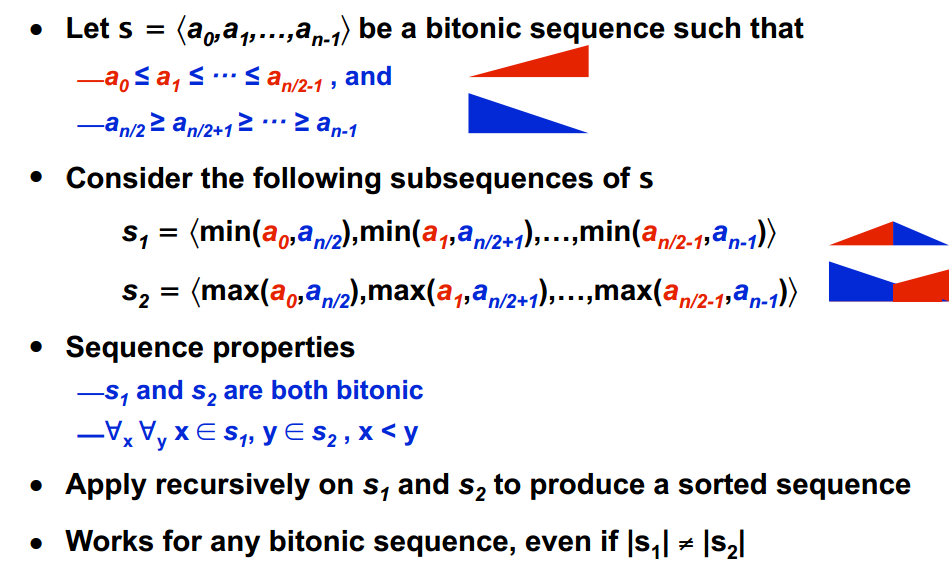
\includegraphics[width=0.5\textwidth]{../figures/bitonic_split.png}
\caption{\label{fig:BitonicSort}Représentation de la logique derrière le tri bitonique.}
\end{figure}
\end{frame}

%%%%%%%%%%%%%%%%%%%%%%%%%%%%%%%%%%%%%%%%%%%%%%%%%%%%%%%%%%%%%%%%%%%%%%%%%%%%%%%
\begin{frame}{Triage - Bitonic sort}
\begin{figure}[h]
\centering
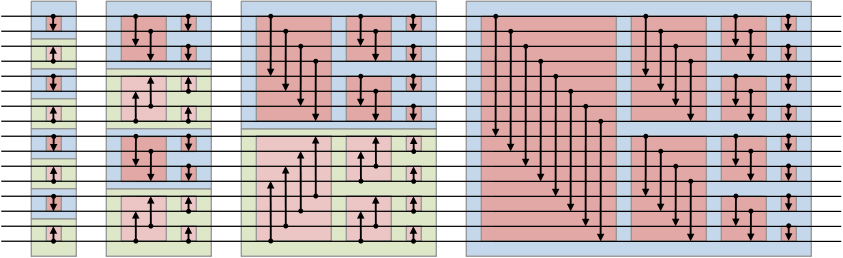
\includegraphics[width=0.6\textwidth]{../figures/BitonicSort1.png}
\caption{\label{fig:BitonicSort}Réseau de tri du tri bitonique.}
\end{figure}
\end{frame}

%%%%%%%%%%%%%%%%%%%%%%%%%%%%%%%%%%%%%%%%%%%%%%%%%%%%%%%%%%%%%%%%%%%%%%%%%%%%%%%
\begin{frame}{Résultats}
\begin{figure}[h]
\centering
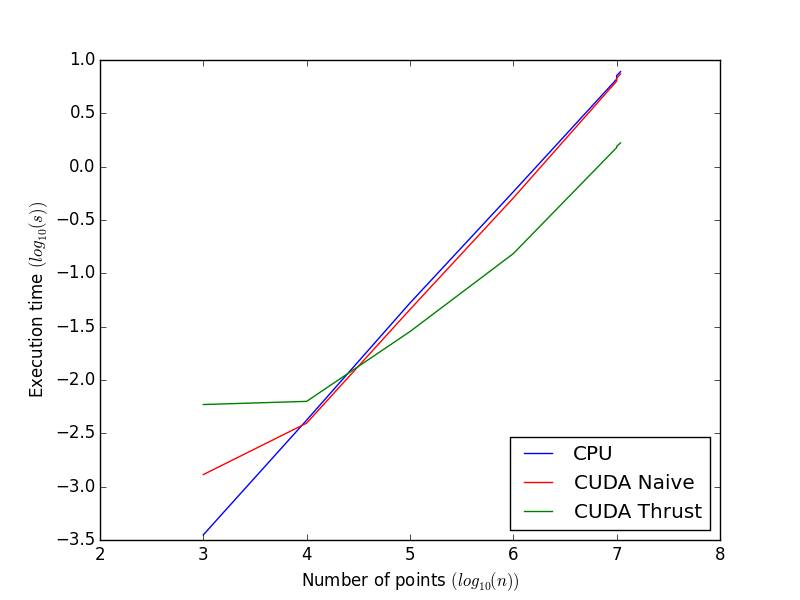
\includegraphics[scale=0.3]{../figures/comparison.jpg}
\caption{\label{fig:Comparaison}Comparaison de temps d'execution sur un \emph{Core i7 4700MQ - GTX850} avec 15 dimensions.}
\end{figure}
\end{frame}

%%%%%%%%%%%%%%%%%%%%%%%%%%%%%%%%%%%%%%%%%%%%%%%%%%%%%%%%%%%%%%%%%%%%%%%%%%%%%%%
\begin{frame}{Autres approches}
\begin{itemize}
\item Odd-Even Merge Sort
\item Heap Sort 
\item Kd-trees
\end{itemize}
\end{frame}

%%%%%%%%%%%%%%%%%%%%%%%%%%%%%%%%%%%%%%%%%%%%%%%%%%%%%%%%%%%%%%%%%%%%%%%%%%%%%%%
\begin{frame}
\begin{center}
\LARGE \textbf{Questions ?}
\end{center}
\end{frame}
\end{document}